Modularization concepts for the process industry increase flexibility. The plant operator is faced with the challenge of no longer being able to solve problems on the basis of extensive experience. Assistance systems can relieve people of many tasks and accompany them through a problem-solving process. The analysis of this thesis shows the complexity of the influencing factors on problem and solution. The user is supported by the interaction platform developed so that he still has an overview at all times. The interaction platform draws attention to the relevant information. Among experts, the simple operation of the system and the clarity of the solutions receives a very positive response and would be recommended by them.

\vspace{10pt}
\begin{center}
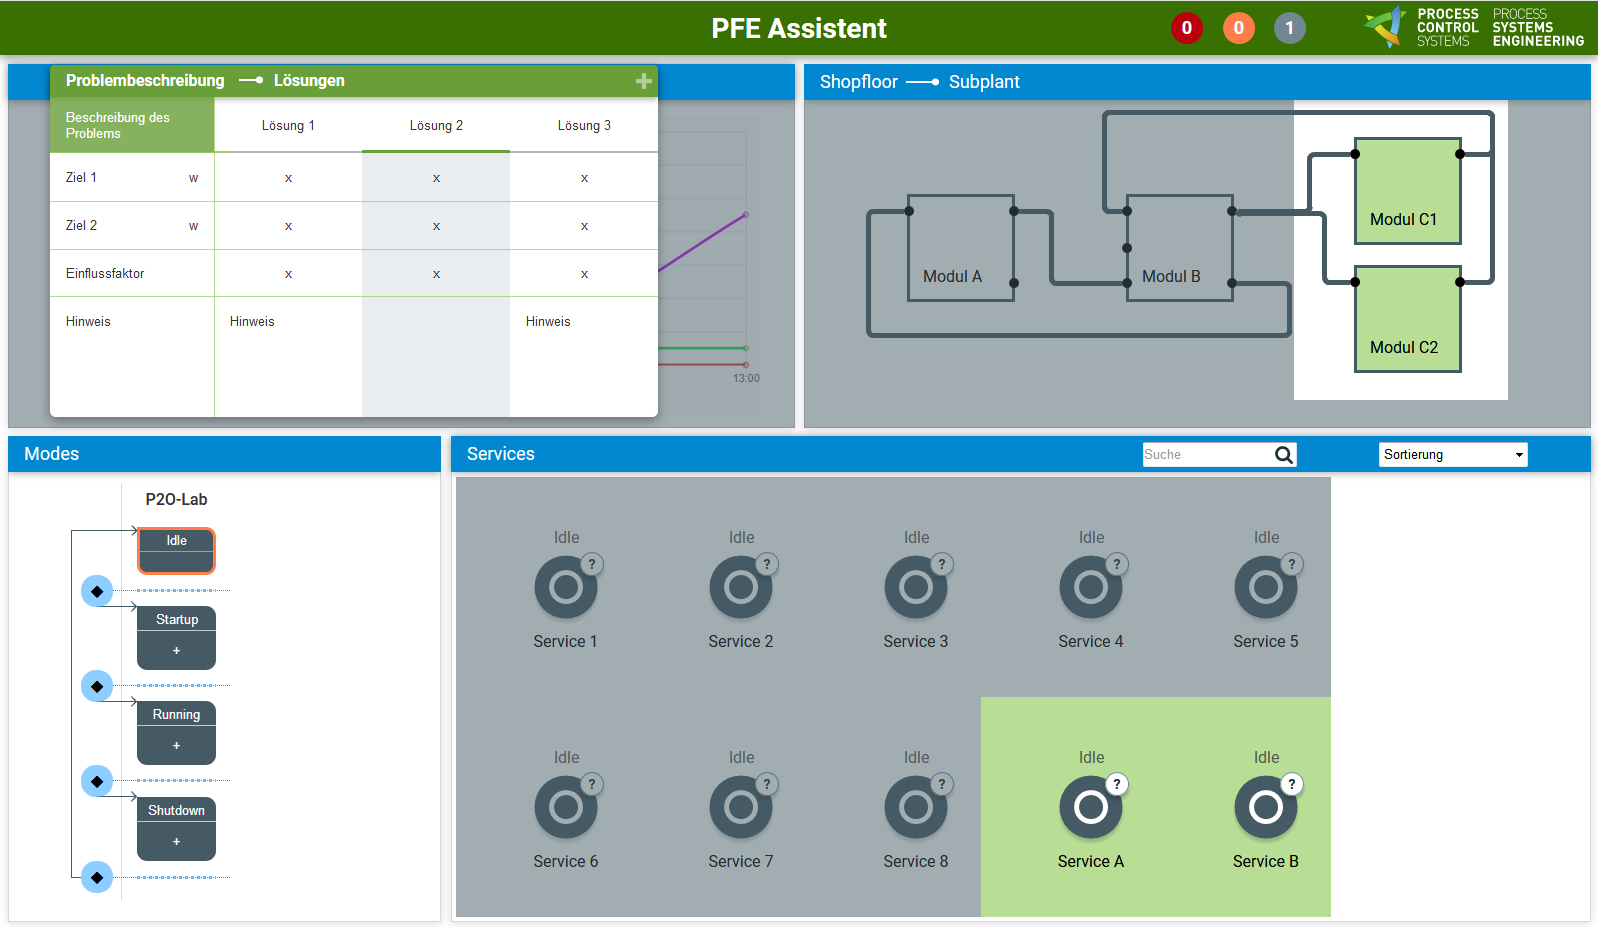
\includegraphics[scale=0.25]{DA_files/Bilder/Konzept/Skizze-Loesungen-PFE.png}
%[keepaspectratio, width=13 cm]
\end{center}
\vspace{6pt}